\documentclass[10pt,conference,compsocconf]{IEEEtran}

\usepackage{hyperref}
\usepackage{graphicx}	% For figure environment

\usepackage{amsmath}
\let\proof\relax
\let\endproof\relax
\usepackage{amsthm}
\usepackage{amssymb}
\usepackage{graphicx}
\usepackage{tikz}
\usetikzlibrary{shapes,arrows}

\usepackage{bm}
\usepackage{amssymb}
\usepackage{diagbox}
\graphicspath{ {images/} }



\def\bN{{\mathbb N}}
\def\bZ{{\mathbb Z}}
\def\bQ{{\mathbb\bf Q}}
\def\cA{{\mathcal A}}
\def\cC{{\mathcal C}}
\def\cE{{\mathcal E}}
\def\cG{{\mathcal G}}
\def\cH{{\mathcal H}}
\def\cI{{\mathcal I}}
\def\cM{{\mathcal M}}
\def\cO{{\mathcal O}}
\def\cU{{\mathcal U}}
\def\b0{{\underline{0}}}
\def\lra{\longrghtarrow}
\def\Lra{\Leftrightarrow}
\def\Ra{\Rightarrow}
\def\lla{\longleftarrow}
\def\la{\leftarrow}
\def\ra{\rightarrow}
\def\wt{\widetilde}
\def\ol{\overline}
\def\tz{\c{t}}
\def\Tz{\c{T}}
\def\sh{\c{s}}
\def\Sh{\c{S}}
\def\ua{\u{a}}
\def\uA{\u{A}}
\def\aa{\^{a}}
\def\AA{\^{A}}
\def\ii{\^{i}}
\def\II{\^{I}}
\def\cart{\times}
\def\pzt{\textbf{p}$_{zt}$}
\def\pzt{\textbf{p}$_{zt}$}
\def\ci{\mathcal{I}}
\def\bR{\mathbb{R}}
\def\bQ{\mathbb{Q}}
\def\vv{\textbf{v}}
\def\xx{\textbf{x}}
\def\zz{\textbf{z}}
\def\id{\mathcal{I}}
\def\eh{\hat{e}}


\begin{document}
\title{Stochastic Accuracy Ascent in the text classification competition}

\author{
	Ciprian Baetu, Doru Musuroi, Joseph Vavala
}

\maketitle

\begin{abstract}
  An important challenge in text classification tasks is obtaining the proper embeddings
  on which the \textit{usual suspects} can be trained. We present in this report
  our work with three types of text embeddings - GloVe, FastText and Sent2vec. We used the mentioned methods to create vector representations for tweets, and afterwards trained, as a baseline, standard Machine Learning algorithms like Logistic Regression and SVM with linear kernel, on the representations. Finally,  we came up to our best-performing model based on a meta ensembling pipeline composed of neural networks as base predictors on top of embeddings and a linear model as the stacking model.
\end{abstract}

\section{Introduction}

Working with textual information in Machine Learning has been a challenge for a long time. Processing text is very different from the other types of information, e.g. images, because the "atom" should be represented by words, but also because there are almost no rules in how those words can be connected in a proper and logical sentence. Also, the usual encoding for images is very natural, such that if you change a single bit in the pixel-matrix representation, we still have a valid encoding, while changing a bit in textual information represented, for the sake of argument, in ASCII code, the whole text might become invalid. \\

Therefore, scientists tried to find a way to represent textual information such that we can apply usual Machine Learning techniques on top of it. A breakthrough has been realized by the creators of word2vec \cite{MCC13+}, which used matrix factorization opposed to neural networks as a main background algorithm for training efficient text representations. After their idea, multiple algorithms based on the same technique were developed, improving the performance of the initial algorithm.\\

The project which we chose to approach was the \textit{Text Sentiment Classification} on Twitter data. The main task of the project is to come up with a solution which predicts if a tweet message contained a positive smile, denoted by \textit{:)}, or a negative smile, marked in text by \textit{:(}. Even though the name suggests that \textit{sentiment classification} should be performed on tweets, the truth is somewhat different: a user might insert a happy face in an ironical manner, even though the sentiment is negative, or there could be just a typo in the tweet, or maybe, as we actually seen in the data, the user starts an enumeration with a colon sign \textit{:} and then opens a bracket for a short explanation. \\

Our approach was a gradual one: the first methods tried are very simple, where we just tuned-in pre-trained existing models on our data and we tried to assess the accuracy using those models. Afterwards, we realized fine-tuning on each method, and finally came up with a solution which stacks multiple classifiers, using predictions from different methods. 

\section{Sent2vec bBseline}
As mentioned in the problem description, our prediction unit was a sentence. This determined us to try Sent2vec\cite{PGJ17}, an unsupervised model developed at EPFL, which produces numerical representations for short texts or sequences. Hence we were able to use the classic and rather fast machine learning algorithms for an initial baseline directly on the output of Sent2vec. 
\subsection{Method description}
Having recently improved the state-of-the art in both unsupervised and semi-supervised models, the main idea of the Sent2vec model is that, for each word in the vocabulary, it learn two embeddings, source and target, improving on the already existing model \cite{MCCD13} by also learning source embedding for word n-grams. The sentence embeddings are then produced by taking the words and word-n-grams in it and averaging over their source embeddings. 

The training set of our task was evenly split into two files with 1.250.000 entries each, where they either contained tweets corresponding to \textit{:)} or to \textit{:(}. Our approach has three steps: first we train the sent2vec model on the 2.500.000 tweets resulted from the concatenation of the two files. Secondly, we produce the sentence-embedding for 100.000 tweets for each label. The resulted 200.000 entries were split 80\%-20\%  train-validation sets on which we trained and evaluated a Logistic Regression model, a Support Vector Machine with linear kernel and a Dense Neural Network. We repeated this pipeline in a grid-search fashion over the parameters of sent2vec in order to obtain the best initial results.
\subsection{Method's results}
In order to find the right sent2vec model, we ran a grid-search over the following parameters:
\begin{itemize}
	\item \textit{dimension of the embeddings} with values between 10, 30, 100 and 300
	\item \textit{n-gram} with values between 1 and 2
	\item \textit{epochs} with values between 10 and 20
\end{itemize}

We observed that the biggest increase in accuracy was due to the dimension of embeddings and the number of n-grams. As the epochs value did not influence the accuracy of the classifiers, in Figure 1 we decided to present the results only for 10 epochs.

\begin{figure}[h]
	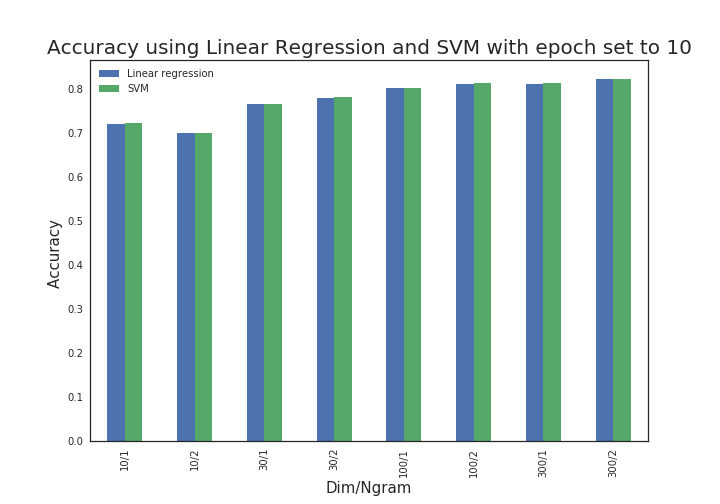
\includegraphics[width=8cm]{LinRegSVMaccuracy2.png}
	\caption{Accuracy results on the sent2vec embeddings of Logistic Regression and SVM}
\end{figure}

We present in table 1 the result of various architectures of Dense Neural Networks on the grid-searched parameters for the Sent2Vec model. As for Logistic Regression and SVM, the variation of epochs parameter did not produce considerable changes in the accuracy.


\begin{center}
	\begin{table}[h]
		\begin{tabular}{|c|*{3}{>{$}c<{$}|}}
			
			\hline
			\diagbox[linewidth=0.2pt, width=0.8 \textwidth/5+5\tabcolsep\relax, height=0.6cm]{$\enspace\boldsymbol Dim/Ngram $}{$\;\boldsymbol NN $}
			& (100)  & (300) & (200,200)\\
			\hline
			$ 10/1 $ & 0.759 & 0.760 & 0.756 \\
			\hline
			$ 30/1 $ & 0.801 & 0.797 & 0.761  \\
			\hline
			$ 30/2 $ & 0.812 & 0.805 & 0.774  \\
			\hline
			$ 100/1 $ & 0.819 & 0.792 & 0.793  \\
			\hline
			$ 100/2 $ & 0.829 & 0.813 & 0.805  \\
			\hline
			$ 300/2 $ & 0.806 & 0.813 & 0.814  \\
			\hline
		\end{tabular}
		\caption{Accuracy obtained for 3 Layers Dense Neural Networks in conjunction with the parameters for sent2vec}
	\end{table}
\end{center}


\section{FastText baseline}
In the same time, we tried to use FastText \cite{JGB16+}, a method developed at Facebook for efficient text classification. As it was mentioned during the course, the method is among the best ones that exist nowadays, therefore that is the reason for trying it for the first time. 

\subsection{Motivation}
As we already mentioned, word2vec represented a breakthrough in the area, allowing  users to construct vector representations, called \textit{embeddings} for words existing in a given text. Interestingly enough, the resulted vectors can also carry some semantics, allowing sum or difference operations over embeddings, with meaningful interpretations. Even though the results are even shocking at a first sight, we can see there is a small flaw: after training the algorithm on a dataset, we cannot retrieve representations for a word which was not previously encountered. Knowing that users tweets are usually not very correctly written, with many typos, slangs and jargons present, we believe that being able to construct representations for words which were not encountered in the training set would be a big plus in this context.\\

This is where fastText comes in handy, because it does exactly what word2vec couldn't handle. More specifically, it also has the option to construct the representation for "\textit{out-of-bag}" words, by constructing embeddings for different parts of words too. Therefore, for a new, unseen word, a representation is done by averaging some of the embeddings for the "sub-words" \cite{BGJ16+}, i.e. small parts of the word. 

\subsection{How does it work?}

But how is fastText working under the hood? It is very interesting to see that the method used is extremely easy, relying again on matrix factorization \cite{LeS00}, as word2vec does. Therefore, given $\mathcal{V}$ the set of all words used for training, and also a tweet written as:
\begin{center}
	$tweet_n = (w_1, w_2,...,w_m)$,
\end{center}

where $w_1,w_2,...,w_m$ are the words of the tweet, we can construct the bag-of-words representation of the tweet as a vector $x_n \in \bR^{\mathcal{|V|}}$. Using this representation, our goal is to find the matrices $W \in \bR^{1\times K}$ and $Z \in \bR^{|\mathcal{V}| \times K}$ that minimize the negative log-likelihood over the output classes: 

\begin{center}
	$\mathcal{L}(W, Z) = - \frac{1}{N} \sum\limits_{n=1}^{N} y_n log (f(WZ^\top x_n))$,
\end{center}

where:

\begin{itemize}
	\item $N$ is the number of tweets in the dataset
	\item $x_n \in \bR^{|\mathcal{V}|}$ is the bag-of-word representation of tweet $n$
	\item $y_n \in \{-1, 1\}$ is the label of tweet $n$
	\item $f$ is the softmax function
\end{itemize}

\subsection{fastText on our dataset}

The results of fastText on our problem are very promising. As we started with an accuracy of around 80\%, we decided to try some parameter tuning in the model. We performed a grid-search on different parameters of the model, as mentioned below:

\begin{itemize}
	\item \textit{dimension of the embeddings}: values between 10, 30, 50 and 100
	\item \textit{number of epochs}: values between 5, 10, 15, 20, 50
	\item \textit{minimum number of word occurrences to be counted}: 1, 5, 10
	\item \textit{"sub-word" size}: (1, 6), (1, 7), (2, 6), (2, 7), where a pair ($x, y$) means that we considered all subwords of length between $x$ and $y$.
	
	\item \textit{n-gram size}: all between 1-7. A n-gram means a pair of $n$ consecutive words, which is actually needed to establish the context for words.  
\end{itemize}

With the results from the grid-search, we decided that the best parameters are: \textit{dimension of the embeddings}: 30, \textit{number of epochs}: 12 (we fine-tuned between 10 and 15), \textit{minimum occurrences}; 1, \textit{subword size}: (2, 7) and \textit{n-gram size}: 6. The rest of the parameters are the default ones in the algorithm made available by Facebook Research team. 

This resulted in an accuracy of 87.02\%, which would have theoretically projected us on the first place in the leaderboard. That was the moment when we decided to create the first submission and to have a skyrocket result. \\

The results were not as high as expected, though, as the kaggle submission accuracy on public leaderboard was 96.3\%, which only helped us to be on the 7th position out of around 50 at that point. This was very disappointing, but we tried to find out reasons for this behavior. We tried several more submission which locally had over 87.8\% accuracy, but on kaggle, the highest accuracy was 86.72\%. We realized there should be a problem causing a difference of over 1\% between local and public score, and we dig into that problem.

\subsection{What was the root source of the big differences?}

We started to perform an exploratory analysis of the data. While doing so, we realized that there were duplicated tweets in the dataset. Trying to get an idea on how many tweets are actually duplicate, we realized that the number of unique tweets on both positive and negative files was about 90\% of the tweets in the entire file. That meant that approximately 10\% of the tweets were repeating, so when we split the dataset into \textit{train} and \textit{test}, there was a non-negligible number of tweets in the test set that were also in the training set.

Looking also into the training accuracy, we realized that it was incredibly high, of more than 99.9\%, which meant that the classifier was overfitting \textit{a lot}, therefore almost all the training instances were perfectly classified by the learned classifier. Therefore, the instances in the testing set that were actually also a part of the training set were a bonus to the accuracy, and that caused our classifier to have such a big difference between the locally computed accuracy and the one on kaggle.

\subsection{What did we decide to do?}

Next, we decided to preprocess the datasets. As we didn't want to spend a lot of time on that, the easiest preprocess we could think of was to remove all the duplicates, and to consider the provided datasets as only containing unique tweets, therefore training on only 90\% of the initial data, but basically the same amount of information in tweets. 

As expected, this decision resulted in having a local test accuracy lower than before, but it was in fact lower than we expected, i.e. less than 86.0\%. Again surprisingly, we had an increase with 0.08\% on public leaderboard, we think because the classifier was not overfitting anymore. 

In all the next submissions, the local accuracy was lower than the one computted on kaggle, therefore we just realized that the local accuracy should be a lower bound for the accuracy we can gain on kaggle. This is most of the times true, as also the test set contains duplicates and because the probability of a duplicate being predicted as correct would be really high, we experience an average increase in accuracy on real test set.\\

What we could have done differently here would have been to try to split the training set and test set such that there were no common tweets, but in the same time keep the same number of occurrences for each tweet. More explicitly, if a tweet appears once in training set, then insert all subsequent tweets equal to that one also in the training set, and the same for the test set. That would mean to create a partition of the data such that we could have preserved the overall distributions, and maybe we would have had a local accuracy closer to the real accuracy on kaggle. This is very interesting to verify from now on on this dataset.  

\subsection{Trying fastText with linear classifiers}

Very interesting, fastText is also able to output embeddings for the whole tweet, and not only for a single word. That's why we thought we can combine the power of fastText embeddings with the power of an external classifier. Therefore, we created representations for the tweets using the best model from before, and then we applied different classifiers on the resulted embeddings, such as Logistic Regression, SVM and K-Nearest Neighbors. The local results were similar to the ones when we used \textit{only} fastText, but we still submitted it to kaggle, and we were sad to see that the accuracy was only 86.5\%, therefore lower than our best accuracy at that point. \\

Also, we tried afterwards to use the pre-trained fastText vectors of dimension 300 which are available online, but also to learn embeddings in an unsupervised manner on the full dataset of tweets \cite{BGJ16+}, and then to apply the usual classifiers mentioned before on the tweets expressed using the created embeddings. All those trials did not lead to a higher local accuracy, so we decided not to continue in this direction anymore.

Finally, we just realized we reached a local maximum with the fastText method, so we decided to move on, and explore further approaches.

\section{GloVe Baseline}

Next, we remembered that also GloVe \cite{PSM14} was mentioned during the course, and that we were provided with a GloVe starting implementation. Therefore, we decided to experiment a little bit using this method.

We chose to use this instead of word2vec because it is unanimously accepted between the scientists in the domain that GloVe provides better embeddings, even though the underlying idea of it is almost the same as for word2vec.  \\

In our implementations, we used the embeddings of dimension 200 available online, pretrained on a \textit{Twitter} dataset. Then, we decided to go further and,  instead of using the basic aforementioned Machine Learning algorithms, to apply neural networks algorithms, using Keras software \cite{Cho15}, as presented in Yoon Kim's paper \cite{Kim14}. \\

The only model we tried in this setup was a simple one, with a Convolutional layer over the embeddings, followed by a MAX pooling layer, again a Convolutional layer followed by the same kind of MAX pooling layer, then another Dense layer with reLu activation function and on the final layer, activation function sigmoid and loss function represented by Binary Crossentropy. The kaggle results with this setup was an accuracy of 86.4\%, which was lower than the one achieved by that point.

\section{Stacking models}
Finally, we decided to use all the aforementioned classifiers into one single, stacked classifier. The idea is pretty simple \cite{Bre96}: each classifier might be able to perform better on specific cases, and we want to use this in our favor. Therefore, what we did was to split all the training data into three folds. For each fold, we trained each classifier on the remaining two folds, and predicted the values for the current fold. In this manner, we would have, for each classifier, a set of predictions for each datapoint in the training set. In the end, we would train each classifier on all training data, and then predict the values of the final test dataset. \\

What we constructed is, in fact, a new dataset, with the same number of instances, but with very few features, i.e. as many as the classifiers used to predict. Now, finally, we could consider another general classifier, such as a Logistic Regression, which can be fitted on the train meta-features created, and then trying to predict the label for each test instance, using the test meta-features. \\

\section{Results}

Finally, we combined 6 base classifiers on the first tier: 
\begin{itemize}
	\item one \textit{fastText} classifier, the one that was performing the best so far
	\item one \textit{sent2vec} classifier, also the best so far
	\item two neural networks with convolutional layers trained on GloVe embeddings, as presented in the previous section
	\item two neural networks as the ones above, but which instead of the second convolutional layer, had a Long-Short Term Memory (LSTM) layer.
	\item the last four classifiers also had a Dropout layer before the last one. 
\end{itemize}

The second tier classifier considered was a Gradient Boosting algorithm, trained on the dataset with 6 features, as we presented above. The final kaggle accuracy is 87.72\%, which makes us to take the 7th position in the public leaderboard. 

\section{Conclusion}

Text analysis is, in general, very difficult to perform, as the natural language does not follow mathematical, strict rules, and is also continuously changing. We achieved an accuracy of 87.72\% on a text classification problem, but this was possible only by using a method which stacks classifiers. However, in real-life problems, people tend to prefer having simpler models, with better interpretability, instead of pushing the limits with several stacked classifiers, but for the purpose of the project, this method had its own gains. 


\bibliographystyle{IEEEtran}
\bibliography{literature}

\end{document}
